\documentclass[a4paper]{article}
\usepackage{graphicx}
\usepackage{amsmath, amsfonts, geometry, float, listings, enumerate, multicol}
\usepackage{multicol, float, color, colortbl}
\usepackage{tikz, titlesec, parskip, pgfplots, filecontents}
\usepackage{hyperref}
\usepackage{amsmath}
\usepackage{tikz, titlesec, parskip}
\usepackage{tikz,pgfplots}
\usepackage[americanvoltages,fulldiodes,siunitx]{circuitikz}
\usetikzlibrary{shapes,arrows}
\usepackage{enumitem}

\titlespacing{\section}{0pt}{10pt}{0pt}
\titlespacing{\subsection}{0pt}{10pt}{0pt}
\titlespacing{\subsubsection}{0pt}{10pt}{0pt}

\usetikzlibrary{calc,patterns,through}
\newcommand{\arcangle}{%
	\mathord{<\mspace{-9mu}\mathrel{)}\mspace{2mu}}%
}

\renewcommand{\baselinestretch}{1.4}
 \geometry{
 a4paper,
 total={170mm,257mm},
 left=20mm,
 top=20mm,
 }
\usepackage{fancyhdr}
\usepackage{indentfirst}
\pagestyle{fancy}
\fancyhf{}
\rhead{\textbf{آمار و احتمال مهندسی}}
\lhead{\textbf{تمرین سری اول}}
\cfoot{(\space \space \space \space \textbf{\thepage}  \space \space \space)}
\renewcommand{\headrulewidth}{1pt}
\renewcommand{\footrulewidth}{1pt}

 
\usepackage{xepersian}
\setlatintextfont{Times New Roman}
\settextfont{XB Niloofar}
\setdigitfont{XB Niloofar}
\DefaultMathsDigits

\makeatletter
\bidi@patchcmd{\@Abjad}{آ}{الف}
{\typeout{Succeeded in changing آ into الف}}
{\typeout{Failed in changing آ into الف}}
\makeatother
\PersianAlphs

\begin{document}
\begin{minipage}{0.6\textwidth}
\begin{bf}
\begin{center}
	به نام خدا\\
	\vspace{0.25cm}
	دانشگاه صنعتی شریف\\
	\vspace{0.25cm}
	دانشکده مهندسی برق\\
	\vspace{0.5cm}

\large
گروه دکتر پاکروان - سیستم‌های مخابراتی \\
نیم سال اول
۱۴۰۱-۱۴۰۰\\
\Large
\vspace{0.4cm}
تمرین عملی سری اول\\
\end{center}
\end{bf}
\normalsize
\end{minipage} \hfill
\begin{minipage}{0.35\textwidth}
\begin{flushleft}
\includegraphics[width=0.6\textwidth]{Shariflogo.png}\\ \large
\end{flushleft}

 \end{minipage}
\\

\rule[0.1\baselineskip]{\textwidth}{1.5pt}

\large

\section*{
لطفاً به نکات زیر توجه بفرمایید:
}
\begin{enumerate}
	\item 
نتایج و پاسخ های خود را در یک فایل با فرمت zip به نام
\LR{HW$1$-Name-StudentNumber}
 در سایت  cw قرار دهید.
	\item 
کسب نمره کامل در هر سؤال مستلزم تحویل  \textbf{کدها} و \textbf{توضیحات} می‌باشد. 
\item 
برای سؤالات، باید روشی که استفاده کرده‌اید را توضیح  و نتایجی که گرفته‌اید را ارائه دهید. این توضیحات می‌تواند در یک فایل  pdf باشد.
\item 
کدهای خود را خوانا بنویسید و کامنت‌‌گذاری کنید.
\item
ابهام يا اشكالات خود را مي توانيد  از طریق
\href{https://t.me/Amirhosein_javadi}{@Amirhosein\_Javadi}
یا 
\href{mailto:javadiamirhosein.2000@gmail.com}{\LR{Javadiamirhosein.$2000$@gmail.com}}
مطرح نماييد.
\item 
کدهای شما تماماً باید توسط خودتان نوشته شده باشند. هرگونه استفاده از کد دیگران به هر شکل ممکن، تقلب محسوب می‌شود و نمره تمرین کامپیوتری جاری صفر خواهد شد. پس در هیچ صورت کدهای خود را برای دیگران ارسال نکنید.

\item 
مهلت تحویل:  
\end{enumerate}
\clearpage
 	
\section{
تاثیر کانال چند مسیره
}
سیگنال $ x(t) $ را به صورت زیر در نظر بگیرید:
\begin{equation}
			 x(t) =  cos(2 \pi  f_{0} t)	\quad (f_{0}  = 2)
\end{equation}
\begin{enumerate}
	\item 
	این سیگنال را برای 10 ثانیه در نظر بگیرید و نمونه برداری کنید. سپس سیگنال را در حوزه زمان رسم کنید.
	\\
حال میخواهیم اثر یک کانال چند مسیره را روی شکل موج بررسی کنیم. فرض کنید سیگنال ارسال از طریق $ 10 $ مسیر به مقصد میرسد. پس پاسخ ضربه سیستم برابر است با: 
\begin{equation}
	\begin{split}
		h(t)_{Channel} =  \sum_{i=1}^{10} a_{i} \delta(t-\tau_{i})
		\\
		H(f)_{Channel} =  \sum_{i=1}^{10} a_{i} e^{-j2 \pi f \tau_{i}}
	\end{split}
	\label{channel}
\end{equation}
برای طراحی کانال ضرایب $ a_{i} $ ها را به صورت تصادفی از توزیع رایلی با پارامتر $ \sigma = 0.5 $ و  $ \tau_{i} $ ها را به صورت تصادفی از توزیع یکنواخت در بازه‌ی $ [0,0.01] $ انتخاب کنید.
\item
یک کانال به این صورت تولید کنید و اندازه و فاز پاسخ فرکانسی آن را رسم کنید.
\item
دره‌های موجود در اندازه پاسخ فرکانسی را در نظر بگیرید. فاصله این دره‌ها با پارامتر‌های کانال رابطه‌ای دارند؟ توضیح دهید.
(برای اطلاعات بیشتر میتوانید درباره‌ی notch در پاسخ فرکانسی مطالعه کنید.)
\item
حال سیگنال را $ 10 $ بار در کانال تصادفی ارسال کنید و هر بار پاسخ ضربه را به صورت بالا تولید کنید. سپس خروجی‌های این  $ 10 $ کانال را پشت سر هم قرار دهید و در حوزه‌ی زمان رسم کنید و تغییرات تصادفی توان سیگنال را مشاهده کنید.
\end{enumerate}
\section{
بازیابی سیگنال خروجی از کانال چند مسیره
}
همان‌طور که در بخش قبل دیدید کانال چند مسیره باعث میشود سیگنال دریافتی  distorted شود. در این بخش سعی می‌کنیم سیگنال اصلی را بازیابی کنیم.
\\
کانال ایده‌آل به صورت زیر است:
\begin{equation}
	 H(f)_{Ideal} = k e^{-j2 \pi f t_{0}} 
\end{equation}
ولی به دلیل رسیدن موج از چند مسیر، کانال به شکل معادله‌ی 
 \ref{channel}
است. به منظور بازیابی سیگنال ورودی دقیق در گیرنده‌، از Equalizer استفاده می‌شود به گونه‌ای که کل عملکرد سیستم را می توان به عنوان یک کانال ایده‌آل مدل کرد.
\\
اگر پاسخ فرکانسی سیستم‌ Equalizer را $ H(f)_{Equalizer}  $ بنامیم، داریم:
\begin{equation}
	H(f)_{Ideal} = H(f)_{Equalizer} \; H(f)_{Channel} 
\end{equation}
پس در صورتی که $  H(f)_{channel}  $ را داشته باشیم میتوانیم $ H(f)_{Equalizer}  $  را طراحی کنیم:
\begin{equation}
	H(f)_{Equalizer} = \dfrac{H(f)_{Ideal}}{ H(f)_{channel} } = \frac{k e^{-j2 \pi f t_{0}}}{\sum_{i=1}^{n} a_{i} e^{-j2 \pi f \tau_{i}}}
\end{equation}
برای مدل‌سازی این سیستم فرض می‌کنیم $ t_{0} = \tau_{1} $ و $ k = a_{1} $ ، پس داریم: 
\begin{equation}
	H(f)_{Equalizer} = \frac{1}{1+\sum_{i=2}^{n} \dfrac{a_{i}}{a_{1}} e^{-j2 \pi f (\tau_{i}-\tau_{1})}} = \frac{1}{1+\sum_{i=2}^{n} k_{i} e^{-j2 \pi f t_{i}}}
\end{equation}
که
  $ k_{i} = \dfrac{a_{i}}{a_{1}} $
  و 
  $ t_{i} = \tau_{i}-\tau_{1} $
  است. 
  \\
  در صورتی که 
  $ \lvert \sum_{i=2}^{n} k_{i} e^{-j2 \pi f t_{i}} \rvert < 1 $
  باشد میتوانیم با بسط تیلور با متناهی جمله، $ H(f)_{Equalizer} $ را با دقت بالا تقریب بزنیم:
\begin{equation}
  	H(f)_{Equalizer} = \frac{1}{1+\sum_{i=2}^{n} k_{i} e^{-j2 \pi f t_{i}}}  \approx 1 + \sum_{k=1}^{m} \big(-\sum_{i=2}^{n} k_{i} e^{-j2 \pi f t_{i}}\big)^{k}
  	\label{Equalizer}
\end{equation}
هر جمله ی پاسخ فرکانسی بالا متناسب با یک شیفت زمانی با ضریب مخصوص به خود است.
 \\
 به این روش برای بازیابی سیگنال خروجی  
\textbf{ \LR{Tapped-Delay Line Equalizer}}
 میگوییم که ساختاری به شکل زیر دارد:
 
 \begin{figure}[H]
 	\begin{center}
 		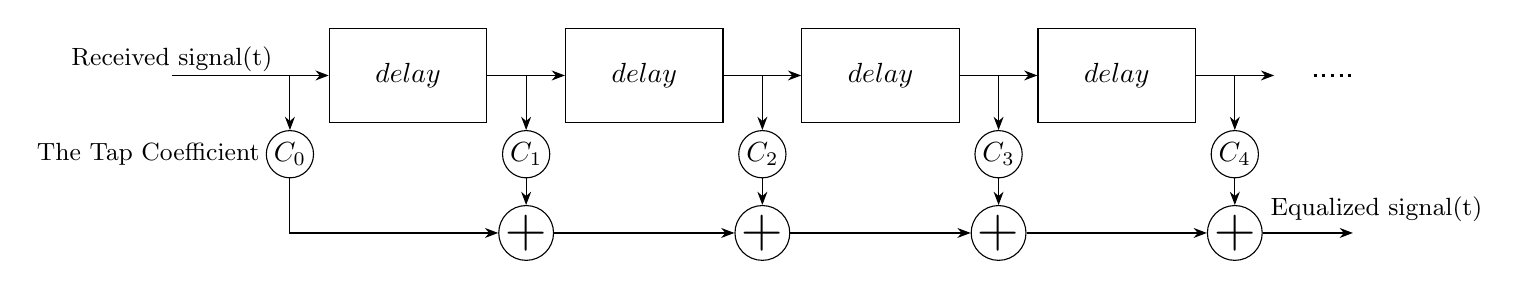
\begin{tikzpicture}
 			[
 			block/.style={draw, minimum width=20mm, minimum height=12mm},
 			sum/.style={circle, draw, minimum size=6mm, inner sep=0pt,
 				node contents={\huge$+$}},
 			mult/.style={circle, draw, minimum size=6mm, inner sep=0pt},
 			>=Stealth,
 			node distance=12mm and 10mm]
 			\coordinate (in) at (-2,0) [];
 			\node (delay1) [block]  at (1,0) {$delay$};
 			\node (delay2) [block]  at (4,0) {$delay$};
 			\node (delay3) [block]  at (7,0) {$delay$};
 			\node (delay4) [block]  at (10,0) {$delay$};
 			\coordinate (node1) at (12,0) [];
 			\coordinate (out) at (13,-2) [];
 			\node (m1)  at (-0.5,-1) [mult] {$C_{0}$};
 			\node (m2)  at (2.5,-1) [mult] {$C_{1}$};
 			\node (m3)  at (5.5,-1) [mult] {$C_{2}$};
 			\node (m4)  at (8.5,-1) [mult] {$C_{3}$};
 			\node (m5)  at (11.5,-1) [mult] {$C_{4}$};
 			\node (s1)  at (2.5,-2) [sum];
 			\node (s2)  at (5.5,-2) [sum];
 			\node (s3)  at (8.5,-2) [sum];
 			\node (s4)  at (11.5,-2) [sum];
 			\draw[->]   (in) -- (delay1);
 			\draw[->]   (delay1) -- (delay2);
 			\draw[->]   (delay2) -- (delay3);
 			\draw[->]   (delay3) -- (delay4);
 			\draw[->]   (delay4) -- (node1);
 			\draw[->]   (in) -| (m1);
 			\draw[->]   (delay1) -| (m2);
 			\draw[->]   (delay2) -| (m3);
 			\draw[->]   (delay3) -| (m4);
 			\draw[->]   (delay4) -| (m5);
 			\draw[->]   (m1) |- (s1);
 			\draw[->]   (m2) -- (s1);
 			\draw[->]   (s1) -- (s2);
 			\draw[->]   (m3) -- (s2);
 			\draw[->]   (s2) -- (s3);
 			\draw[->]   (m4) -- (s3);
 			\draw[->]   (s3) -- (s4);
 			\draw[->]   (m5) -- (s4);
 			\draw[->]   (s4) -- (out);
 			\draw[scale=1,dotted,line width = 0.4mm,black] (12.5,0) -- (13,0);
 			
 			\draw (-2.3,-1) node[centered]  {\small The Tap Coefficient};
 			\draw (-2,0.2) node[centered]  {\small Received  signal(t)};
 			\draw (13.3,-1.7) node[centered]{\small Equalized signal(t)};
 		\end{tikzpicture}
 		\caption{\LR{Tapped-Delay Line Equalizer}}
 	\label{system}
\end{center}
\end{figure}
حال می‌خواهیم با این روش یک سیگنال خروجی از کانال چند مسیره را بازیابی کنیم. سیگنال ورودی را به صورت زیر در نظر بگیرید:
\begin{equation}
	x(t) =  cos(2 \pi  f_{0} t) (u(t)-u(t-2))	\quad (f_{0}  = 2)
\end{equation}
\begin{enumerate}
	\item 
این سیگنال را برای 10 ثانیه در نظر بگیرید و نمونه برداری کنید. سیگنال را در حوزه‌ی زمان نشان دهید.
\\
پاسخ ضربه کانال را به صورت زیر تعریف کنید:
\begin{equation}
	h(t) =  \delta(t-5) + 0.4\delta(t-5.01)
\end{equation}
	\item 
اندازه‌ و فاز پاسخ فرکانسی کانال را رسم کنید.

	\item 
سیگنال را از این کانال بگذرانید و سیگنال خروجی را در کنار سیگنال ورودی در حوزه‌ی زمان نشان دهید.
	\item 
حال میخواهیم سیگنال ارسالی را از سیگنال خروجی کانال به دست بیاوریم. برای این کار میزان خطا را به شکل زیر تعریف کنید:
\begin{equation}
	error =  \frac{rms(Equalized \; signal - Ideal \; received \; signal)}{rms( Ideal \; received \; signal)}
\end{equation}
	که 
	\LR{Equalized  signal}
	سیگنالی است که شما بازسازی می‌کنید و 
	\LR{Ideal received signal}
	سیگنال شیفت یافته ارسالی به اندازه‌ی 5 ثانیه است.
	حال با استفاده از فورمول \ref{Equalizer} میزان خطا را به ازای 
	$ m = 1:10 $
	به دست بیاورید و روی یک صفحه نیمه لگاریتمی نشان دهید.
	\item
	حال در یک صفحه سیگنال دریافتی، سیگنال ایده‌آل دریافتی و سیگنال   Equalized را نشان دهید.
\end{enumerate}

\end{document}
